\section{Solid breeder background}\label{sec:intro-blanket-description}

The solid breeder blanket is an integral part of the power generation and fuel cycle in a fusion reactor. On the road to understanding the specific functional requirements of the solid breeder blanket, we will review the major features of a fusion reactor power and fuel cycle as they relate to the blanket. Currently, the worldwide choice for fusion reaction in a power plant is the deuterium-tritium (DT) reaction. The choice is based on DT having: a high reaction probability at the lowest ion temperature, high energy yield, availabile fuel (to a degree), and relatively harmless reaction products. The DT reaction is
\begin{align}
	\mathrm{D} + \mathrm{T}&\xrightarrow{}~^4\mathrm{He}+\mathrm{n}+17.58~\text{MeV} \label{eq:dt-reaction}
\end{align}

Of the two isotopes fused, deuterium ($D$, or $^2$H) is a stable isotope and is naturally occuring in an average abundance of 0.015 mole percent in water on Earth. But tritium ($T$, or $^3$H), contrarily, is radioactive with a half-life of only about 12.32 years; naturally decaying as a $\beta^-$ emitter,
\begin{align}\label{eq:t-decay}
	\mathrm{T} \xrightarrow{}~^3\mathrm{He} + \beta^-
\end{align}

Owing to its short half-life, any naturally occurring tritium decays at such a rapid pace it will never accumulate to an appreciable amount on Earth. Because of this, to use the DT reaction in a fusion power plant, tritium will need to be generated artificially (bred) and collected as fuel source. One way of breeding tritium for a fusion reactor is to include a so-called tritium breeding blanket that surrounds the fusion plasma with a phase of lithium. We will keep our focus completely on the solid, non-mobile choice of a lithium blanket but note that lithium as a liquid is also heavily studied as a potential tritium breeding blanket.

The two most abundant isotopes in natural lithium interact with the neutrons as given in Eq.\ref{eq:lithium-t}
\begin{subequations}\label{eq:lithium-t}
\begin{align}
	\mathrm{n} + ~^7\mathrm{Li} &\xrightarrow ~\mathrm{n}+\alpha + \mathrm{T} -2.47~\text{MeV}\label{eq:li7-t}\\
	\mathrm{n} + ~^6\mathrm{Li} &\xrightarrow ~ \alpha + \mathrm{T} +4.78~\text{MeV} \label{eq:li6-t}
\end{align}
\end{subequations}
where we haved used the common short-hand of $\alpha$ in place of the helium nucleus. The cross-sections of the lithium reactions are given in Fig.~\ref{fig:li-xsects}. Note the exothermic lithium-6 reaction and the threshold energy required of the incident neutron to incite the lithium-7 reaction.

\begin{figure}
	\centering
	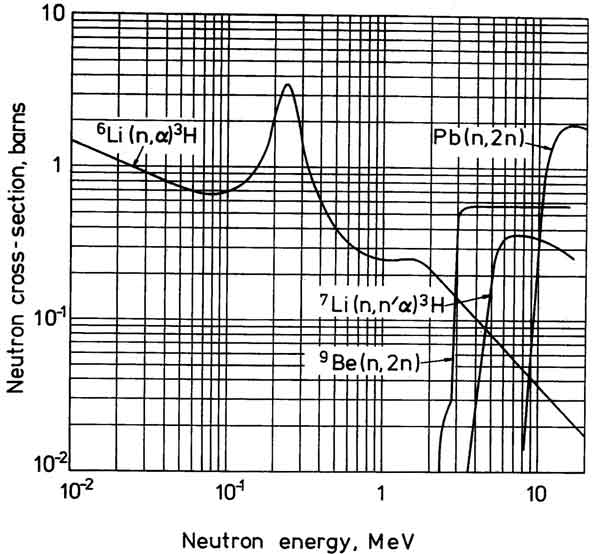
\includegraphics[width=0.75\textwidth]{chapters/figures/breeding_xsecs} 
	\caption{Cross-sections of various blanket materials. Note the threshold for the $^7$Li and neutron multiplying reactions.}
	\label{fig:li-xsects}
\end{figure}

Serendipitously, the DT reaction itself produces a high energy neutron (see Eq.~\ref{eq:dt-reaction}) that can interact with the two isotope reactions of Eq.~\ref{eq:lithium-t}. Therefore sulf-sufficiency of the fusion fuel cycle can be realized with the fusion neutron interacting with the lithium blanket. A commonly used classification of the efficacy of a breeding blanket is via the tritium breeding ratio (TBR), defined as 
\begin{equation}
	\text{TBR} = \cfrac{\dot{N}^+}{\dot{N}^-}
\end{equation}
where $\dot{N}^+$ is the number of tritium atoms generated per unit time in the blanket and $\dot{N}^-$ are the number of tritium atoms consumed per unit time.

For a DT cycle that creates a single neutron we can simplify this definition to say the tritium breeding ratio is the number of tritium atoms produced in the blanket per fusion neutron. If every single neutron from the fusion reaction were to be captured by lithium, we would have a TBR of $\approx 1$ and the reactor would possibly be self-sufficient in this ideal case. Unfortunately, in reality, only 60-80\% of the fusion neutrons actually react with the lithium due to neutron leakage and parasitic reactions. Futhermore, when we take into account tritium retention in structural material or losses due to inefficiency in collecting tritium, then self-sufficiency of the fuel cycle is clearly not possible unless we produce more than one tritium per fusion neutron. 

For solid breeders, beryllium is introduced into the blanket as a neutron multiplier. The incident neutron breaks Be up into two $\alpha$ particles and an additional two neutrons. Thus it is possible, with careful neutronics analysis and engineering of tritium breeding volumes and neutron multiplying regions, to attain a TBR which makes the power plant not only self-sufficient in terms of fuel, but also able to seed tritium for a future power plant. Assuming that the fuel cycle of tritium is handled properly (perhaps the biggest assumption we will make in this work), the last remaining function of the blanket is to supply energy for the electricity generation of the power plant. 

The fusion reaction deposits a great deal of surface radiation on the first wall of the breeding blanket and the blanket will be absorbing energy deposited from neutron interactions and $\gamma$ rays. The blanket must be capable of converting and then recovering the energy at high tempreatures for efficient power production in the fusion power plant. The nuclear heat generated in the pebble bed solid breeder will heat the ceramic pebbles to maximum temperatures of approximately 900~\celsius. The heat of the pebbles is transported through them via conduction through inter-particle contacts, conduction through the purge gas into neighboring particles, and ultimately through contact with the containing structure. The box structure surrounding the solid breeder will have high pressure (\si{8~MPa} in many current designs) helium flowing through channels that remove the heat from the blanket, with the helium reaching temperatures of 500~\celsius, and into a power generation cycle.

In summary, it is feasible, in principle, for a fusion power plant to produce electricity and be self-sustaining in terms of its limiting fuel. The feasibility depends on the the ability engineer a device that surrounds the fusion reaction, captures the ejected neutron to breed tritium, allows recovery of that tritium to attain self-sufficiency, and delivers the energy deposited in the blanket as high quality heat into a power cycle to create electricity. Blanket designs of solid breeders have evolved significantly since their introduction in the 1970s. Some features of current breeder designs will be discussed next.
%~~~~~~~~~~~~~~~~~~~~~~~~~~~~~~~~~~~~~~~~~~~~~~~~



%~~~~~~~~~~~~~~~~~~~~~~~~~~~~~~~~~~~~~~~~~~~~~~~~
\subsection{Solid breeder material and form considerations}
Pure lithium has a melting temperature of only about 180~\celsius so must be combined with a refractory material to keep it in solid form at high temperatures (melting temperatures >1000~\celsius). To date, most parties researching solid breeder blankets are focusing on lithium orthosilicate (\lis) or lithium metatitanite (\lit) as candidate ceramics, though other candidate ceramics do still exist. Lithium oxide had been considered because of its favorable lithium density, among other attractive features, though the reaction of lithium with elemental oxygen is a concern. Pure lithium reacts with oxygen exothermically in reactions such as

\begin{subequations}
\begin{align}
	2\mathrm{Li} + \frac{1}{2}\mathrm{O} &\rightarrow \mathrm{Li}_2\mathrm{O} - 142.75~\text{kCal/mol}\\
	2\mathrm{Li} + \mathrm{O} &\rightarrow \mathrm{Li}_2\mathrm{O}_2 - 151.9~\text{kCal/mol}
\end{align}
\end{subequations}

Of primary concern in lithium fires is the peak flame temperature. This will determine, to a large extent, whether many radioactive species become air-borne by vaporization. The flame temperature depends on many variables. Some investigations found it to be about 2500~K which would cause some materials to melt but not vaporize. [cite Abdou's class notes?]

As nuclear energy is deposited into the solid breeder, large thermal gradients in the solid lithiated ceramics will induce thermal stresses across large characteristic lengths. Avoiding thermal stress has led to most solid breeder designs implementing packed beds of small, spherical (or near-spherical) pebbles. Moreover, tritium diffusion and release considerations for solid lithium ceramic support the choice of short characteristic lengths of individual pebbles. From an engineering design standpoint, the choice of packed bed has other desirable characteristics. For instance, the ensemble of small spherical pebbles can be filled into many complex shapes with relatively uniform porosity for well-distributed flow of the purge gas. 

The packed bed will be contained in a structure of ferritic or austenitic steel. The energy of the packed bed is carried away by coolant channels in the structure that have flowing in them high pressure helium gas. Because the structural material is held cooler than the breeding zone, it will confine the thermal expansion of the lithium ceramic and lead to mechanical stresses at the points of contact of the individual pebbles in the packed bed. Engineering design issues surrounding this thermal stress is of great concern to researchers and will be the focus of much of this report.

Once in operation, the ceramic pebble beds will have a specified operating temperature window that is dictated by tritium release characteristics. The low end of the temperature window is governed by a minimum temperature for acceptable release rates of tritium from the ceramic to the purge gas; the value is generally set around 500~K. The upper limit of the temperature window is chosen to avoid sintering of the lithiated ceramic. Sintering of the ceramics, as grains in individual pebbles meld, is predicted to reduce the rate of tritium release. The upper end of the temperature window is generally set around 1000~K.

The size of breeder regions is limited by the temperature window combined with the poor effective conductivity of packed beds of ceramic pebbles. The conductivity is a weak function of external pressure but can generally be approximated as about \si{1 W/{mK}}. Because the effective conductivity and packed bed-wall interface conductance is predominately a contact conduction, disruptions to the packing structure will have considerable impact on the heat transfer of the packed bed.

As each individual tritium breeding region is small, in a typical solid breeder blanket design there are several alternating layers of breeding zone, cooling plate, and neutron multiplier. 

The two most prominently analyzed neutron multipliers for a fusion reactor are beryllium and lead. Beryllium has a very high nuclide density while also being very light, with a high melting temperature, and high thermal conductivity. For solid breeding blankets, beryllium has been pegged as the element of choice. The beryllium, based on its own design requirements, is generally also chosen to exist in a pebble bed form in the breeding blanket device.

